\section{Reproducible experiments and negative controls}\label{sec:experiments}

\subsection{Protocol and interpretation}

The raw evidence contains the complete tested face pairings, cocycles, caps,
operation counters, completed certificates and independent replay results.
Experiments used Python 3.12.14; the optional external topology audit used
Regina 7.4. Timings were collected in a shared execution environment without
CPU isolation. They are descriptive measurements on the declared examples,
not estimates of an asymptotic exponent or population-wide performance.

The geometric benchmark has one warm-up pair and three recorded pairs per
size, with seeded randomized arm order. It reports the median of the three
within-pair naive/sleep ratios. The LP audit has three alternating-order
pairs per case and reports the ratio of the two arm medians. These statistics
are intentionally named separately: they need not give the same number.
Neither protocol warrants narrow confidence intervals from three repetitions.
Raw observations allow a later isolated rerun and a different statistical
analysis without reconstructing the sources.

\subsection{Finite completeness and independently checked geometry}

The geometric audit compares naive, commitment and sleep exploration on
eleven small marked instances, including bounded upward search, relabelling,
protected initial cells and a 2,048-bit marking. Together with the maintained
coherent obstruction, it records 34 search calls. There are no endpoint-set
mismatches among the three methods on the finite comparisons.

An independent endpoint checker accepts 91 audit certificates; 90 targeted
mutations are rejected. These include changes that would falsify source
protection or the upward allowance, in addition to geometric and marking
corruptions. A separate replay of the geometric timing file accepts all 126
saved endpoint certificates. The benchmark timings exclude this later
external replay, but include transition validation and certificate copying
performed by the search itself.

The optional Regina audit examines 23 distinct triangulation states and
176 replacements. It checks the eligible move inventory and the isomorphism
signature of each resulting triangulation. No inventory or replacement
mismatch is observed. This is an independent finite check of the repository's
formal move interpretation; it does not replace the general relative-boundary
proof or certify an untested parameter range.

The new focused tests also compare the canonical-parent region enumerator
with powerset enumeration on every labelled simple graph with at most four
vertices and on three structured six-vertex graphs, across all relevant size
and component caps. They test loops, duplicate adjacencies, validation,
cancellation and callback exception identity. The diagram adapter tests
source mismatch and corrupted proof rejection with the existing checker.
The additional region-and-diagram audit supplies executable small examples
of the union-of-regions semantics: five cases are compared with 120 literal
allowed-subset searches, with 302 successful endpoint replays and no
endpoint or aggregate-count mismatch. Nine diagram calls yield four
independently replayed positive proofs, and three wrong-source substitutions
are rejected. The four positives use two diagram sources under different
options and have zero Pachner moves. They validate the source adapter, not
additional discovery through moves.

There is also an explicit limited-family miss. The two-strand closure of
the word $[1,-1,1]$ is an unknot, since the first two generators cancel.
With boundary shelling enabled and the allowed initial region empty, the
adapter exhausts its declared region family and returns
\status{INCONCLUSIVE}. This small control makes the coverage restriction
observable in executable data. It is not a lower bound for nonempty regions.

\subsection{Independent collapse regions: a geometric control}

For each tested $p=1,\ldots,6$, the driver starts with a layered solid torus
on $2p$ tetrahedra and applies $2$--$3$ moves in $p$ disjoint pairs. The
result has $3p$ tetrahedra and carries the transported cocycle. Its tested
downward event inventory consists of the $p$ independent inverse moves;
the audit also checks that no additional downward event appears at later
endpoints. This realizes the hypotheses of the operation-count calculation
in Section~\ref{sec:commitments} at each reported size.

\begin{table}[tbp]
\centering
\small
\setlength{\tabcolsep}{4pt}
\caption{Genuine independent-collapse controls. Times are medians in milliseconds; the final column is the median within-pair ratio.}
\label{tab:geometric}
\begin{tabular}{@{}rrrrrrr@{}}
\toprule
$p$ & $t$ & $N_{\rm naive}$ & $N_{\rm sleep}$ & Naive (ms) & Sleep (ms) & Paired ratio\\
\midrule
1 & 3 & 2 & 2 & 1.273 & 1.453 & 0.876\\
2 & 6 & 5 & 4 & 13.195 & 10.386 & 1.270\\
3 & 9 & 16 & 8 & 40.916 & 22.266 & 1.838\\
4 & 12 & 65 & 16 & 212.168 & 59.087 & 3.593\\
5 & 15 & 326 & 32 & 1,260.972 & 158.664 & 8.346\\
6 & 18 & 1,957 & 64 & 9,224.509 & 415.842 & 22.183\\
\bottomrule
\end{tabular}
\par\smallskip
\begin{minipage}{0.97\textwidth}
\footnotesize One warm-up pair is excluded. Three measured pairs per size; seeded randomized arm order. Full sources and certificates are saved.
\end{minipage}
\end{table}


At $p=6$, the unreduced search visits 1,957 trace nodes and sleep search
visits 64. The median recorded times are 9.225 and 0.416 seconds, and the
median paired speedup is $22.18$. The gain grows with the repeated-order
work removed in this control. At $p=1$, both methods visit two nodes and
sleep bookkeeping makes the measured time slightly worse. This regression
is retained rather than removed from the comparison.

The distinction between the proof algorithm and the practical algorithm is
large. On the $p=2$ control, full commitment enumeration visits 175,905
assignment frames, whereas the sleep search has four trace nodes. Restricting
the permitted originals to one three-tetrahedron inverse-move region reduces
the commitment search to 401 frames. These are different units of work, but
they show why the constant-alphabet encoding should not itself be sold as a
fast practical traversal. The sleep method inherits its bound without paying
for most inert assignments.

The maintained eight-tetrahedron coherent obstruction supplies a different
control. Sleep exploration finds an independently verified disc after one
downward move and two endpoint queries. This confirms that the implemented
search can escape that particular fixed-triangulation coherent obstruction.
It establishes neither a worst-case locality bound nor a robust timing gain
over the incoming greedy transport code.

\subsection{Exact LP reuse on genuine triangulations}

The LP audit contains fifteen cases and 45 paired samples, hence 90 arm
runs. Each arm has a 35-second wall allowance. The figure-eight cases also
have a 600-pivot allowance. No arm hits the wall allowance. Of the 45 pairs,
36 complete on both sides and have byte-equal certificates. All 21 completed
genuine-triangulation pairs independently verify in both arms. The other
15 completed pairs are the explicitly substituted algebraic controls.

\begin{table}[tbp]
\centering
\small
\setlength{\tabcolsep}{4pt}
\caption{Exact LP screening on genuine triangulations. Each paired entry is baseline/screened; times are seconds.}
\label{tab:lp-genuine}
\begin{tabular}{@{}lrrrrl@{}}
\toprule
Source & LP calls & Pivots & Median seconds & Ratio & Result\\
\midrule
Layered, 1 tet. & 3/3 & 7/7 & 0.001/0.001 & 0.927 & +\\
Layered, 2 tet. & 7/6 & 59/50 & 0.018/0.016 & 1.171 & +\\
Layered, 4 tet. & 15/10 & 354/264 & 0.356/0.267 & 1.332 & +\\
Layered, 6 tet. & 23/14 & 1,073/784 & 2.105/1.559 & 1.350 & +\\
Layered, 8 tet. & 31/18 & 2,620/1,948 & 9.682/8.151 & 1.188 & +\\
Branching torus & 41/22 & 1,134/648 & 1.684/0.908 & 1.855 & +\\
Finite trefoil & 20/20 & 1,554/1,554 & 2.397/2.445 & 0.981 & 0\\
Figure-eight, frozen & 2/2 & 600/600 & 3.872/4.054 & 0.955 & cap\\
Figure-eight, relabelled & 2/2 & 600/600 & 3.976/3.995 & 0.995 & cap\\
Figure-eight, native & 1/1 & 600/600 & 4.358/4.121 & 1.057 & cap\\
\bottomrule
\end{tabular}
\par\smallskip
\begin{minipage}{0.97\textwidth}
\footnotesize $+$: completed positive-Euler query; $0$: completed negative positive-Euler query; cap: inconclusive at 600 pivots. Three alternating-order pairs per case; ratio of arm medians. The result concerns the stated surface query, not an unauthenticated knot-diagram verdict.
\end{minipage}
\end{table}


The branching solid torus is the strongest genuine example in this small
cohort. Calls fall from 41 to 22, pivots from 1,134 to 648, and median elapsed
time from 1.684 to 0.908 seconds. Fifteen omissions come from the pinned
current witness and four from other verified antichain witnesses. This shows
that cross-query reuse can help beyond local zero support.

The layered family gives smaller improvements. At eight tetrahedra, calls
fall from 31 to 18 and pivots from 2,620 to 1,948; the median-time ratio is
$1.19$. The one-tetrahedron case makes the same three LP calls and seven
pivots, so added validation and cache management produce a small slowdown.
The finite trefoil similarly makes the same 20 calls and 1,554 pivots, with
a median-time ratio of $0.98$. Its completed negative certificate remains
exactly equal to the baseline's. A negative result for this positive-Euler
surface query should not be relabelled as a new general knot-recognition
algorithm.

\subsection{Figure-eight controls expose the unsolved cost}

The frozen figure-eight exterior, its relabelled copy, and a regenerated
native finite figure-eight exterior all remain inconclusive at 600 pivots.
There are no screenable deletion queries in these runs. The frozen versions
start two LPs before the allowance is consumed; the native source consumes
it in its first LP. Thus the new cache does not address the current-node
LP bottleneck observed here.

The native fixture is reconstructed with Regina's figure-eight example,
conversion to a finite triangulation, and simplification. Its full face
pairings, version and isomorphism signature are saved. Within each pair the
two producers receive exactly the same reconstructed source. Fresh
simplification need not produce the same combinatorial triangulation, even
within the same Regina version. Reproduction therefore validates each fresh
source without requiring its signature to equal the frozen source's.
The saved native signature is
\begin{center}\code{kLLLALkIcegfegjijjhqhaxrlmlf}.\end{center}

Wall-time differences between two capped, inconclusive runs are not evidence
of faster completed recognition. They remain in the raw data and the table
to show both the resource boundary and the absence of witness hits.

\subsection{The algebraic separation, measured and proved}

\begin{table}[tbp]
\centering
\small
\setlength{\tabcolsep}{4pt}
\caption{Algebraic controls, with no asserted triangulation realization. Every call and pivot total agrees with the proved formula.}
\label{tab:lp-algebraic}
\begin{tabular}{@{}rrrrr@{}}
\toprule
$s$ & LP calls (base/screen) & Pivots (base/screen) & Median seconds & Ratio\\
\midrule
1 & 6/3 & 10/4 & 0.002/0.001 & 1.756\\
2 & 17/5 & 62/14 & 0.018/0.005 & 3.732\\
4 & 57/9 & 436/52 & 0.411/0.053 & 7.781\\
6 & 121/13 & 1,410/114 & 2.677/0.249 & 10.771\\
8 & 209/17 & 3,272/200 & 10.793/0.706 & 15.289\\
\bottomrule
\end{tabular}
\par\smallskip
\begin{minipage}{0.97\textwidth}
\footnotesize Both producers complete with the same substituted algebraic certificate. Ratios are baseline median divided by screened median.
\end{minipage}
\end{table}


Every measured call count agrees with Theorem~\ref{thm:lp-family}. The exact
pivot induction in Appendix~\ref{sec:pivot-appendix} proves, for this solver
and model ordering,
\[
 P_{\rm base}(s)=6s^3+3s^2+s,\qquad
 P_{\rm screened}(s)=3s^2+s.
\]
At $s=8$, this is 209 versus 17 LP calls and 3,272 versus 200 pivots, with a
measured median-time ratio of $15.29$. This is a rigorous cubic-to-quadratic
pivot separation for the algebraic family, supported by finite controls.
It is not a proved cubic-to-quadratic bit-time theorem for arbitrary simplex
tableaux, and it does not supply a triangulation realizing the family.

\begin{figure}[tbp]
\centering
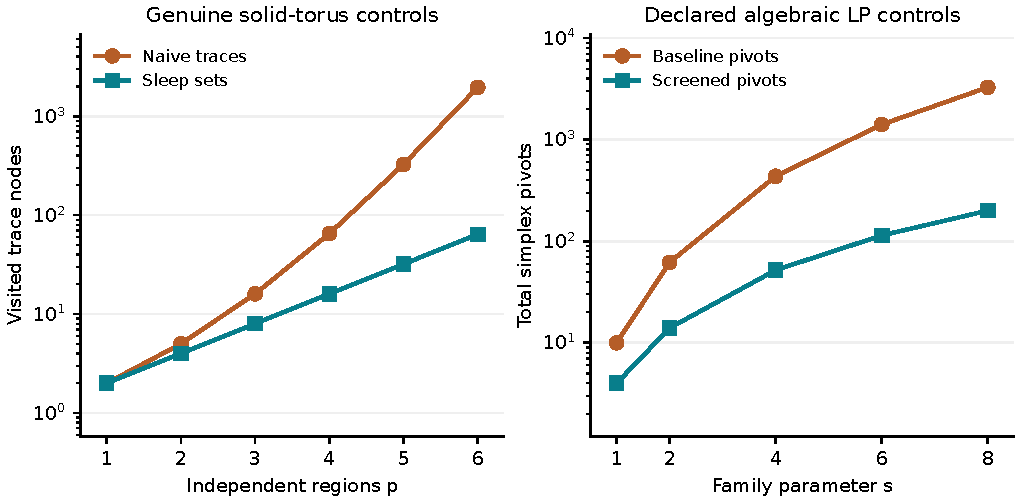
\includegraphics[width=\textwidth]{figures/performance.pdf}
\caption{Measured operation counts on the two controlled families. Left:
actual triangulations with independently collapsible regions, showing all
prefixes before and after sleep reduction. Right: the declared algebraic
LP family, showing exact total pivot counts. Logarithmic vertical axes are
used only for readability. Curves connect the tested integer sizes; the
formulas and their hypotheses, rather than these plots, establish the
asymptotic statements.}
\label{fig:performance}
\end{figure}

\subsection{What the evidence supports}

The geometric result is complete search of a declared finite move family,
with independent replay and a genuine example of factorial ordering
redundancy. The LP result is proof-preserving query omission, with moderate
genuine-triangulation gains and a stronger isolated algebraic separation.
The source adapter gives independently replayed positive diagram verdicts.
None of these observations establishes that every unknot has a successful
small-region trace, that every negative instance is settled by bounded
coherent search, or that exact node LPs have polynomial complexity.

The inherited and added regression tests are covered by the full inventory
gate described in Section~\ref{sec:reproduction}. The archive preserves its
logs, source digests and all failed or interrupted preliminary runs rather
than replacing them with the final successful summary.
